\scanpage{204}
\mspage{-2.3-}
% archive sheet number: 203
ii) for fixed $x$ and $\handwritten{\lambda}$, $\handwritten{\mu}^{L}(x,\handwritten{\lambda})$ defines a homomorphism from $\operatorname{Pic}^{\handwritten{G}}(X)$ to $\handwritten{\mathbb{Z}}$ as $L$ varies.

iii) If $f:X\handwritten{\longrightarrow}Y$ is a $G$-linear morphism of schemes on which $G$ acts, $L\handwritten{\unsure{\in|\epsilon}}\operatorname{Pic}^{\handwritten{G}}(Y)$ and $x\handwritten{\in}X_{\handwritten{k}}$, then
\[
\handwritten{\mu}^{f*L}(x,\handwritten{\lambda})=\handwritten{\mu}^{L}(fx,\handwritten{\lambda}).
\]

iv) If $\handwritten{\sigma(\lambda(\alpha)},x)\handwritten{\longrightarrow}y$ as $\handwritten{\alpha\longrightarrow}0$, then $\handwritten{\mu}^{L}(x,\handwritten{\lambda})=\handwritten{\mu}^{L}(y,\handwritten{\lambda})$.

(Proofs Immediate).

The theorem which we shall ultimately prove is:

\uline{Theorem} \uline{2.1}: Let a \uline{reductive group} $G$ act on a scheme $X$, proper over $k$. Let $L\handwritten{\in}\operatorname{Pic}^{\handwritten{G}}(X)$, and assume $L$ is \uline{ample}. Then if $x\handwritten{\in}X_{\handwritten{k}}$:
% The underlines beneath "reductive group" and "ample" are handwritten and wavy.
\[
\begin{aligned}
x\handwritten{\in}X^{ss}(L)&\handwritten{\Longleftrightarrow}\handwritten{\mu}^{L}(x,\handwritten{\lambda})\handwritten{\geq}0\quad\text{for all 1-PS's }\handwritten{\lambda}\ ,\\
x\handwritten{\in}X^{s}_{(0)}(L)&\handwritten{\Longleftrightarrow}\handwritten{\mu}^{L}(x,\handwritten{\lambda})>0\quad\text{for all 1-PS's }\handwritten{\lambda}\ .
\end{aligned}
\]

There are two approaches to the proof of this theorem. Either we choose a $G$-linear immersion $X\handwritten{\subset\mathbb{P}_{n-1}}$, and reduce to the case $X=\handwritten{\mathbb{P}_{n-1}}$ by Theorem \figure{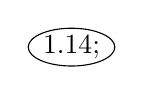
\begin{tikzpicture}[baseline=(a.base)]\node[inner sep=2pt] (a) {1.14;};\draw (a.center) ellipse[x radius=.55cm,y radius=.24cm];\end{tikzpicture}} or we can put $Y$ equal to the normalization of the closure of $\unsure{O|0}(x)$, and via the canonical $\handwritten{\pi}:Y\handwritten{\longrightarrow}X$, reduce to the case where $O(x)$ is dense in $X$ by Theorem \figure{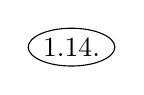
\begin{tikzpicture}[baseline=(a.base)]\node[inner sep=2pt] (a) {1.14.};\draw (a.center) ellipse[x radius=.55cm,y radius=.24cm];\end{tikzpicture}} We shall follow the former which is more down to earth. Therefore \uline{we may assume} $X=\handwritten{\mathbb{P}_{n-1}}$. Now let
% The two ovals and the underline beneath "we may assume" are handwritten.
% margin note written slanted, beside the first reference to Theorem 1.14
\margin{\handwritten{\unsure{why|w}??\\1.19\ \uline{\unsure{2|?}}}}
% right margin: pencil strokes beside "reduce to" and "follow", then an upward arrow and question mark
\figure{\begin{tikzpicture}[x=1cm,y=1cm]
\draw (0,2.2)--(.2,2.15)--(.34,1.97) (.15,2.07)--(.31,2.18);
\draw (0,1.7)--(.4,1.65) (.1,1.72)--(.06,1.52);
\draw (.1,1.2)--(.4,1.15) (.24,1.18)--(.23,.98);
\draw[->] (.23,0)--(.23,.65);
\node at (.8,.65) {\handwritten{?}};
\end{tikzpicture}}
\[
\begin{aligned}
V&=H^{\unsure{0|o}}(\handwritten{\mathbb{P}_{n-1}},\underline{o}(1))\\
\handwritten{\mathbb{A}}^{n}&=\handwritten{\mathbb{V}}(V):\text{ the affine cone over }\handwritten{\mathbb{P}_{n-1}}\ .
\end{aligned}
\]
There is a natural projection from $\handwritten{\mathbb{A}}^{n}-(0)$ to $\handwritten{\mathbb{P}_{n-1}}$. We shall say
